% Informe de avance del proyecto integrador PEU-CD (INEI) para el docente.
% Compilar: pdflatex avance_proyecto.tex (dos veces, para el índice y las referencias cruzadas)
\documentclass[11pt,a4paper]{article}
\usepackage[utf8]{inputenc}
\usepackage[T1]{fontenc}
% Si babel-spanish está instalado se usa; si no (TinyTeX mínimo), se definen los nombres en español a mano.
\IfFileExists{spanish.ldf}{\usepackage[spanish,es-noshorthands]{babel}}{%
  \AtBeginDocument{\renewcommand{\contentsname}{Índice}\renewcommand{\tablename}{Tabla}%
  \renewcommand{\figurename}{Figura}\renewcommand{\refname}{Referencias}}}
\usepackage{lmodern}
\usepackage[margin=2.3cm]{geometry}
\usepackage{graphicx}
\usepackage{booktabs}
\usepackage{tabularx}
\usepackage{longtable}
\usepackage{array}
\usepackage[table]{xcolor}
\usepackage{enumitem}
\usepackage{caption}
\usepackage{float}
\usepackage{tikz}
\usetikzlibrary{arrows.meta,positioning,shapes.geometric,fit}
\usepackage{fancyhdr}
\usepackage[hidelinks]{hyperref}

% Generado a partir de data/huellas/vivo.json y dashboard/data/inundacion.json (recálculo del 4/11/2026)
\newcommand{\VivoEstado}{\hecho}
\newcommand{\VivoTexto}{%
La capa de agua nueva de los últimos 24 días se recalculó con Sentinel-1 después de corregir el error E4.
Usó una referencia seca del 1/8 al 10/10/2026 (42 pasadas) y un evento del 11/10 al 4/11/2026 (13 pasadas, del 12/10 al 2/11).
\begin{itemize}
\item \textbf{Detección:} 334,8 km² en bruto dentro de la caja de estudio; quedan \textbf{27,2 km²} en tierra de Tumbes y Piura después de aplicar las máscaras. El 77\,\% está en Sechura.
\item \textbf{Exposición:} 24 personas y 8 edificaciones dentro de la mancha; ningún colegio ni establecimiento de salud dentro.
\item \textbf{Umbral:} el umbral automático de Otsu, calculado como diagnóstico, fue $-16{,}8$~dB, muy cercano al umbral fijo de $-17$~dB.
\end{itemize}
Es temporada seca, así que el agua nueva corresponde sobre todo a riego y humedales, no a desbordes. La capa pasa el control de calidad y su estado es \emph{vigente}.}


\definecolor{azul}{HTML}{0B3D5C}
\definecolor{ok}{HTML}{1B7F4B}
\definecolor{parc}{HTML}{A35D00}
\definecolor{mal}{HTML}{B3261E}
\newcommand{\hecho}{\textcolor{ok}{\textbf{Hecho}}}
\newcommand{\parcial}{\textcolor{parc}{\textbf{Parcial}}}
\newcommand{\nohecho}{\textcolor{mal}{\textbf{No hecho}}}
\newcommand{\cod}[1]{\texttt{\small #1}}
\newcolumntype{Y}{>{\raggedright\arraybackslash}X}
\renewcommand{\arraystretch}{1.18}
\setlist{itemsep=2pt,topsep=3pt}
\captionsetup{font=small,labelfont=bf}

\pagestyle{fancy}\fancyhf{}
\lhead{\small Proyecto integrador PEU-CD · INEI}
\rhead{\small Informe de avance}
\cfoot{\small \thepage}

\begin{document}

\begin{titlepage}
\centering
\vspace*{2cm}
{\large Instituto Nacional de Estadística e Informática (INEI)\\[2pt]
Programa de Extensión Universitaria en Ciencia de Datos (PEU-CD)\par}
\vspace{2.5cm}
{\LARGE\bfseries\color{azul} Exposición potencial a inundaciones asociadas a El Niño en Tumbes y Piura\par}
\vspace{0.6cm}
{\Large Informe de avance del proyecto integrador\par}
\vspace{2.5cm}
{\large Equipo: Christopher, Maykol, Marcia y Luz Ángela\par}
\vspace{0.4cm}
{\large Corte del avance: 4 de noviembre de 2026\par}
\vfill
{\small Repositorio: \cod{github.com/MarciaShapiama/iapn-inei}\ Tablero: \cod{marciashapiama.github.io/iapn-inei}\\
Todas las cifras se reproducen con \cod{python src/etl.py local} y se verifican con \cod{python -m pytest}.\par}
\end{titlepage}

\tableofcontents
\newpage

\section*{Resumen del avance}
\addcontentsline{toc}{section}{Resumen del avance}

El proyecto busca cuantificar, \textbf{por distrito (UBIGEO)}, cuánta población, cuántas edificaciones, colegios y establecimientos de salud de Tumbes y Piura están \textbf{potencialmente expuestos} a inundaciones. Considera dos fuentes: escenarios de crecida de ríos con periodo de retorno de 10 y 100 años (JRC) y el agua detectada por el radar Sentinel-1 en 2017, 2023 y en los días recientes. Los resultados se publican en un tablero estático, reproducible y con trazabilidad de cada cifra.

En esta etapa:
\begin{enumerate}
\item \textbf{auditamos} el tablero que ya tenía el equipo y encontramos 17 problemas, entre ellos uno crítico: la población estaba desplazada unos 7,9 km;
\item \textbf{corregimos} las cifras y documentamos cuánto cambió cada una;
\item construimos un \textbf{producto mínimo viable} con ETL, metadatos, un mapa 2D sin GPU, un panel de decisiones y 38 pruebas automáticas;
\item \textbf{reprodujimos y evaluamos con rigor} el modelo de machine learning;
\item redactamos los documentos de aporte al INEI, estado del arte y políticas públicas.
\end{enumerate}

\begin{table}[H]\centering\small
\caption{Cifras principales tras las correcciones (zona inundable de 1 en 100 años, JRC). Exposición potencial, no personas afectadas.}
\begin{tabular}{lrl}\toprule
Indicador & Valor & Definición \\\midrule
Superficie inundable & 3\,793 km² & solo dentro de Tumbes y Piura \\
Población potencialmente expuesta & 399\,506 & WorldPop 2026 (modelada) \\
Edificaciones potencialmente expuestas & 148\,348 & Google Open Buildings v3 \\
Locales escolares dentro / hasta 1 km & 682 / 2\,633 & padrón ESCALE (MINEDU) \\
Alumnos en locales dentro & 124\,385 & Censo Educativo 2025 \\
Establecimientos de salud dentro / hasta 1 km & 145 / 577 & RENIPRESS (SUSALUD) \\
Distritos con prioridad alta de revisión & 15 de 76 & índice relativo, no oficial \\\bottomrule
\end{tabular}
\end{table}

\section{Planteamiento}

\paragraph{Problema.} No existe en un solo lugar una cuantificación territorial, reproducible y desagregada por distrito de la exposición a inundaciones en Tumbes y Piura que indique la procedencia y la incertidumbre de cada cifra.

\paragraph{Pregunta.} ¿Cuánta población, cuántas edificaciones y qué servicios esenciales están potencialmente expuestos a inundación fluvial y a las inundaciones detectadas por radar? ¿Qué distritos deberían revisarse primero, considerando a la vez peligro, exposición y vulnerabilidad?

\paragraph{Objetivo general.} Construir y validar un sistema reproducible de indicadores de exposición por UBIGEO, publicado como tablero estático con metadatos y pruebas.

\paragraph{Objetivos específicos.}
\begin{enumerate}
\item Auditar el tablero existente y corregir los errores de cálculo y de rotulado.
\item Calcular la exposición por distrito, dentro de la mancha y en acumulados hasta 500 m y 1 km.
\item Documentar la fuente, la definición, la vigencia y el estado de cada capa.
\item Ofrecer un mapa usable sin aceleración gráfica y descargas abiertas.
\item Evaluar si el machine learning mejora una línea base simple.
\item Proponer un aporte estadístico al INEI y opciones de política pública.
\end{enumerate}

\paragraph{Alcance.} Piloto en Tumbes y Piura (76 distritos en los límites usados; 78 según el INEI). La extensión al resto del Perú queda para una fase posterior.

\section{Cronología del avance}

\begin{table}[H]\centering\small
\begin{tabularx}{\textwidth}{p{2.6cm}Y}\toprule
Fecha & Hito \\\midrule
3 nov.\ 2026 & El equipo inicia el repositorio: monitor del mar (OISST), índices, economía, zonas de lluvia y caudal. \\
3 nov.\ 2026 & Pestaña de inundaciones en 3D: peligro JRC, radar Sentinel-1 2017/2023 y días recientes; exposición de población, edificaciones, colegios y salud. \\
3--4 nov.\ 2026 & Base distrito-semana (DesInventar, NASA POWER, GloFAS) y modelo de alerta con validación por años (42 commits en \cod{main}). \\
4 nov.\ 2026 & \textbf{Auditoría técnica y de datos} (17 hallazgos), corrección de cifras, MVP reproducible, pruebas, recálculo del radar reciente, documentos 01--05, informe final (Word) y este informe de avance (rama \cod{auditoria-mvp-piloto}). \\\bottomrule
\end{tabularx}
\end{table}

\section{Arquitectura}

El sistema no necesita servidor. GitHub Actions descarga y procesa los datos, y GitHub Pages publica archivos JSON/GeoJSON livianos. El costo de operación es cero.

\begin{figure}[H]\centering
\begin{tikzpicture}[node distance=6mm and 8mm, font=\footnotesize,
  caja/.style={draw=azul, rounded corners=2pt, fill=azul!6, align=center, minimum height=8mm, text width=3.1cm},
  dato/.style={draw=gray, fill=gray!8, align=center, minimum height=7mm, text width=3.1cm},
  flecha/.style={-{Stealth[length=2mm]}, thick, azul!70}]
\node[dato] (f1) {NOAA OISST, CPC, IGP\\Open-Meteo, GloFAS};
\node[dato, below=of f1] (f2) {WorldPop, Open Buildings\\RENIPRESS, OSM, GADM, JRC};
\node[dato, below=of f2] (f3) {Sentinel-1 RTC\\(Planetary Computer)};
\node[caja, right=of f1] (d1) {\cod{descargar\_*.py}\\\cod{construir.py}};
\node[caja, right=of f2, text width=3.6cm] (d2) {\cod{exposicion.py}\\\cod{reparar\_poblacion.py}\\\cod{ubigeo.py}};
\node[caja, right=of f3] (d3) {\cod{huellas.py}\\(detección de cambios)};
\node[caja, right=of d2, text width=3.3cm] (imp) {\cod{impacto.py}\\\cod{panel.py}\\\cod{metadatos.py}};
\node[caja, right=of imp, fill=ok!10, draw=ok, text width=3.0cm] (web) {\textbf{GitHub Pages}\\\cod{index.html} (3D)\\\cod{mapa2d.html} (2D)};
\node[caja, above=of web, fill=parc!10, draw=parc, text width=3.0cm] (test) {\cod{tests/} (38)\\Actions «Pruebas»};
\node[caja, below=of web, text width=3.0cm] (reg) {registro y versiones\\(SHA-256)};
\node[draw=azul, dashed, rounded corners, fit=(d1)(d2)(d3)(imp), inner sep=6pt, label={[font=\footnotesize\bfseries,azul]above:\cod{src/etl.py}: reintentos, registro, último válido}] {};
\foreach \a/\b in {f1/d1,f2/d2,f3/d3,d2/imp,d3/imp,imp/web,test/web,imp/reg} \draw[flecha] (\a) -- (\b);
\draw[flecha] (d1.east) -| ([xshift=4mm]imp.north) ;
\end{tikzpicture}
\caption{Flujo de datos. Cada paso deja registro en \cod{data/registro/}. Si una fuente falla, se conserva el último resultado válido y se rotula como «rezagado».}
\end{figure}

\section{Auditoría: qué encontramos y qué corregimos}

\subsection{Hallazgos principales}

\begin{longtable}{p{0.6cm}p{1.4cm}p{6.2cm}p{6.2cm}}
\toprule
ID & Severidad & Problema & Corrección y evidencia \\\midrule\endhead
E1 & Crítica & Población WorldPop desplazada 86 columnas (unos 7,9 km) al oeste: la ventana de recorte salía del borde del ráster de Perú. & Recorte corregido y archivo reparado; correlación con edificaciones de 0,00 a 0,80 (Fig.~\ref{fig:alin}). Prueba automática de alineación. \\
E2 & Alta & Colegios y salud: anillos disjuntos rotulados como acumulados («684 dentro, 1\,268 a $\leq$ 500 m, 684 a $\leq$ 1 km»). & Claves explícitas de anillo y de acumulado; hasta 1 km hay 2\,636 colegios. \\
E3 & Alta & Piura + Tumbes $\neq$ total: faltaban 4\,138 edificaciones fuera de los polígonos distritales. & Fila «Sin distrito asignado»; la suma concilia (prueba). \\
E4 & Alta & Radar «últimos 24 días»: la referencia seca se solapaba con el evento. & Referencia que termina antes del evento; capa recalculada (Sección~\ref{sec:vivo}). \\
E5 & Alta & El radar subdetecta la inundación urbana (Catacaos 2017: 1,1 km²). & Advertencias; plan de validación independiente. \\
E6 & Media & Sin mapa alternativo cuando falla WebGL. & \cod{mapa2d.html} (Leaflet) y detección automática. \\
E7 & Media & Se llamaba «viviendas» a huellas de edificación y se hablaba de «afectados». & Rótulo «edificaciones potencialmente expuestas». \\
E8--E17 & Media/baja & Colegios de OSM con locales de Ecuador; 2 distritos ausentes en GADM; licencia GADM; publicación incompleta en Pages; probabilidades sin calibrar; nombres mal separados; otros. & Documentados en \cod{docs/01\_AUDITORIA\_TECNICA\_Y\_DATOS.md}. \\\bottomrule
\end{longtable}

\begin{figure}[H]\centering
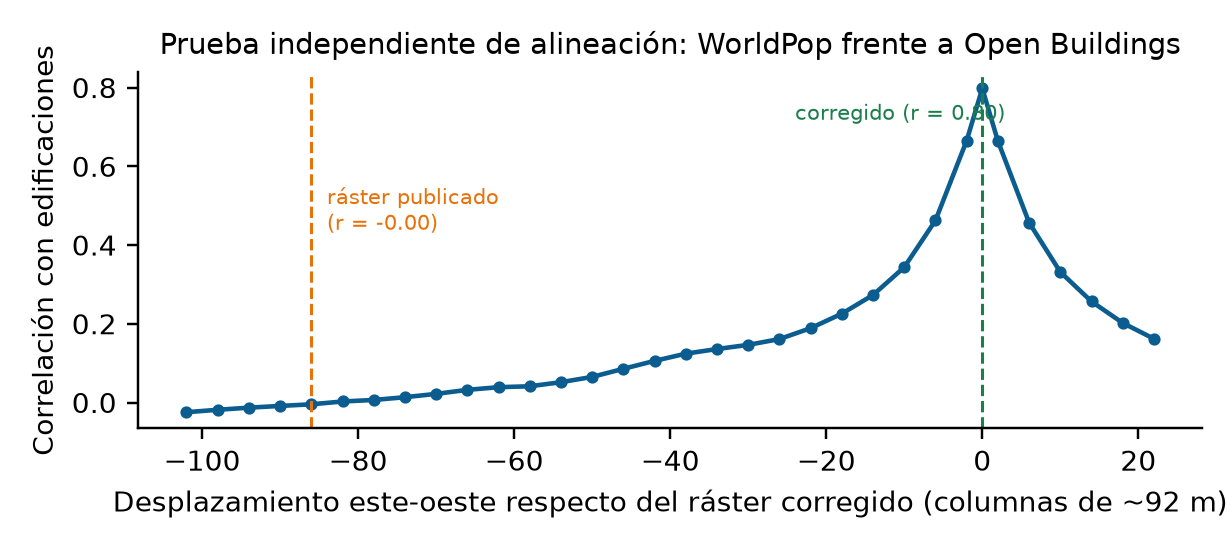
\includegraphics[width=0.86\textwidth]{figuras/alineacion_poblacion.png}
\caption{Prueba independiente de la corrección E1. La correlación entre la población WorldPop y la densidad de edificaciones de Open Buildings es máxima con el ráster corregido y prácticamente nula con el ráster publicado antes.}\label{fig:alin}
\end{figure}

\subsection{Cuánto cambiaron las cifras}

\begin{figure}[H]\centering
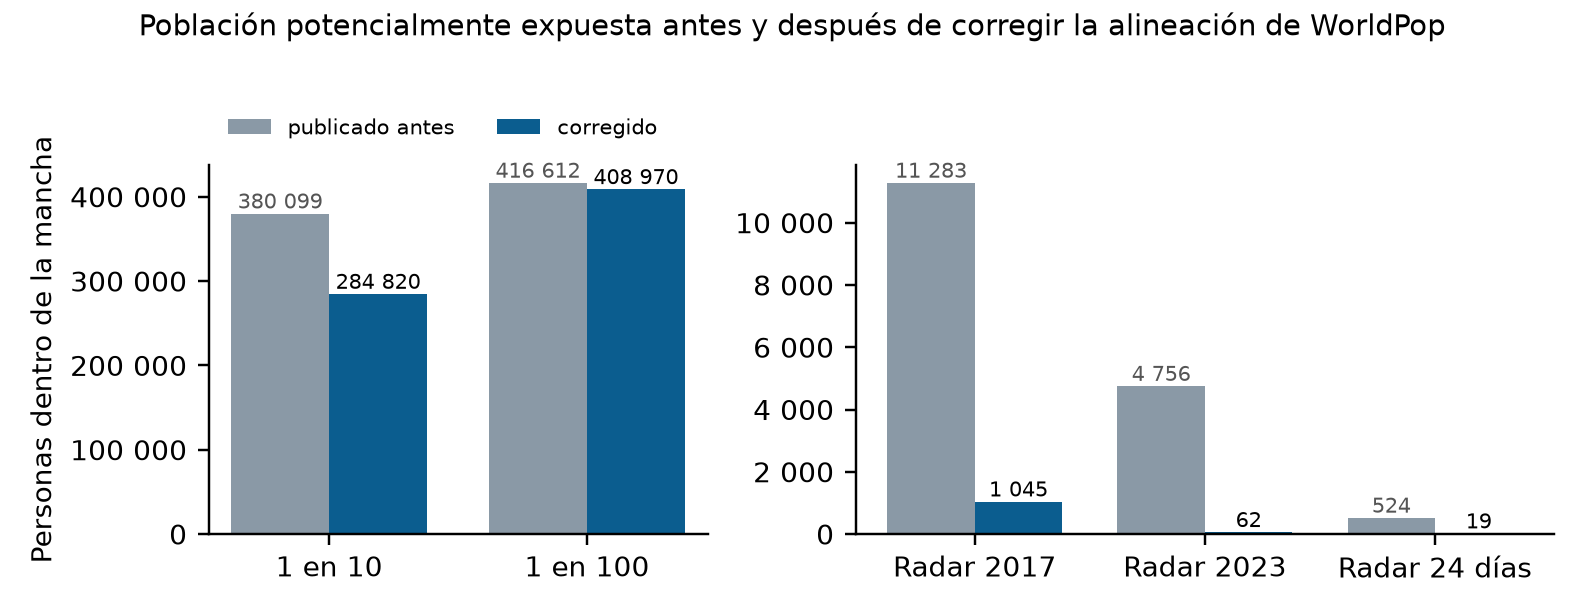
\includegraphics[width=\textwidth]{figuras/antes_despues_poblacion.png}
\caption{Población dentro de la mancha antes y después de la corrección E1. En 2023, la mancha (86\,\% en el desierto de Sechura) tenía en realidad 62 personas, no 4\,756.}
\end{figure}

\subsection{Capa de radar reciente recalculada}\label{sec:vivo}
\VivoTexto

\section{Producto mínimo viable}

\begin{itemize}
\item \textbf{ETL reproducible} (\cod{src/etl.py}) con perfiles \cod{local}, \cod{diario} e \cod{inundacion}. Hace descargas con reintentos y espera exponencial, registra cada corrida, guarda un manifiesto SHA-256 de versiones, escribe los archivos de forma atómica y se configura con variables de entorno.
\item \textbf{Metadatos y estado por capa} (\cod{metadatos.json}): fuente, licencia, definición, unidades, cobertura, resolución, versión, periodo, frecuencia, método, advertencias y estado (\emph{vigente}, \emph{rezagado}, \emph{no disponible}, \emph{estimado}). El estado se calcula con la fecha real del dato.
\item \textbf{Cifras por UBIGEO} (\cod{exposicion\_distritos.csv}): dentro, anillos y acumulados hasta 500 m y 1 km, conciliadas con el total.
\item \textbf{Mapa 2D accesible} sin GPU. Tiene selectores por departamento, provincia, distrito y ámbito de cuenca; escenarios 1/10 y 1/100 y radar 2017/2023/reciente; capas, leyenda, escala, comparador temporal con la fecha de cada pasada, ficha territorial y descargas CSV/GeoJSON. Funciona en celular.
\item \textbf{Panel de decisiones}: peligro, exposición, vulnerabilidad y riesgo estimado en columnas separadas. El riesgo estimado es un índice relativo para priorizar revisiones, no una evaluación oficial (Fig.~\ref{fig:mapa}).
\end{itemize}

\begin{figure}[H]\centering
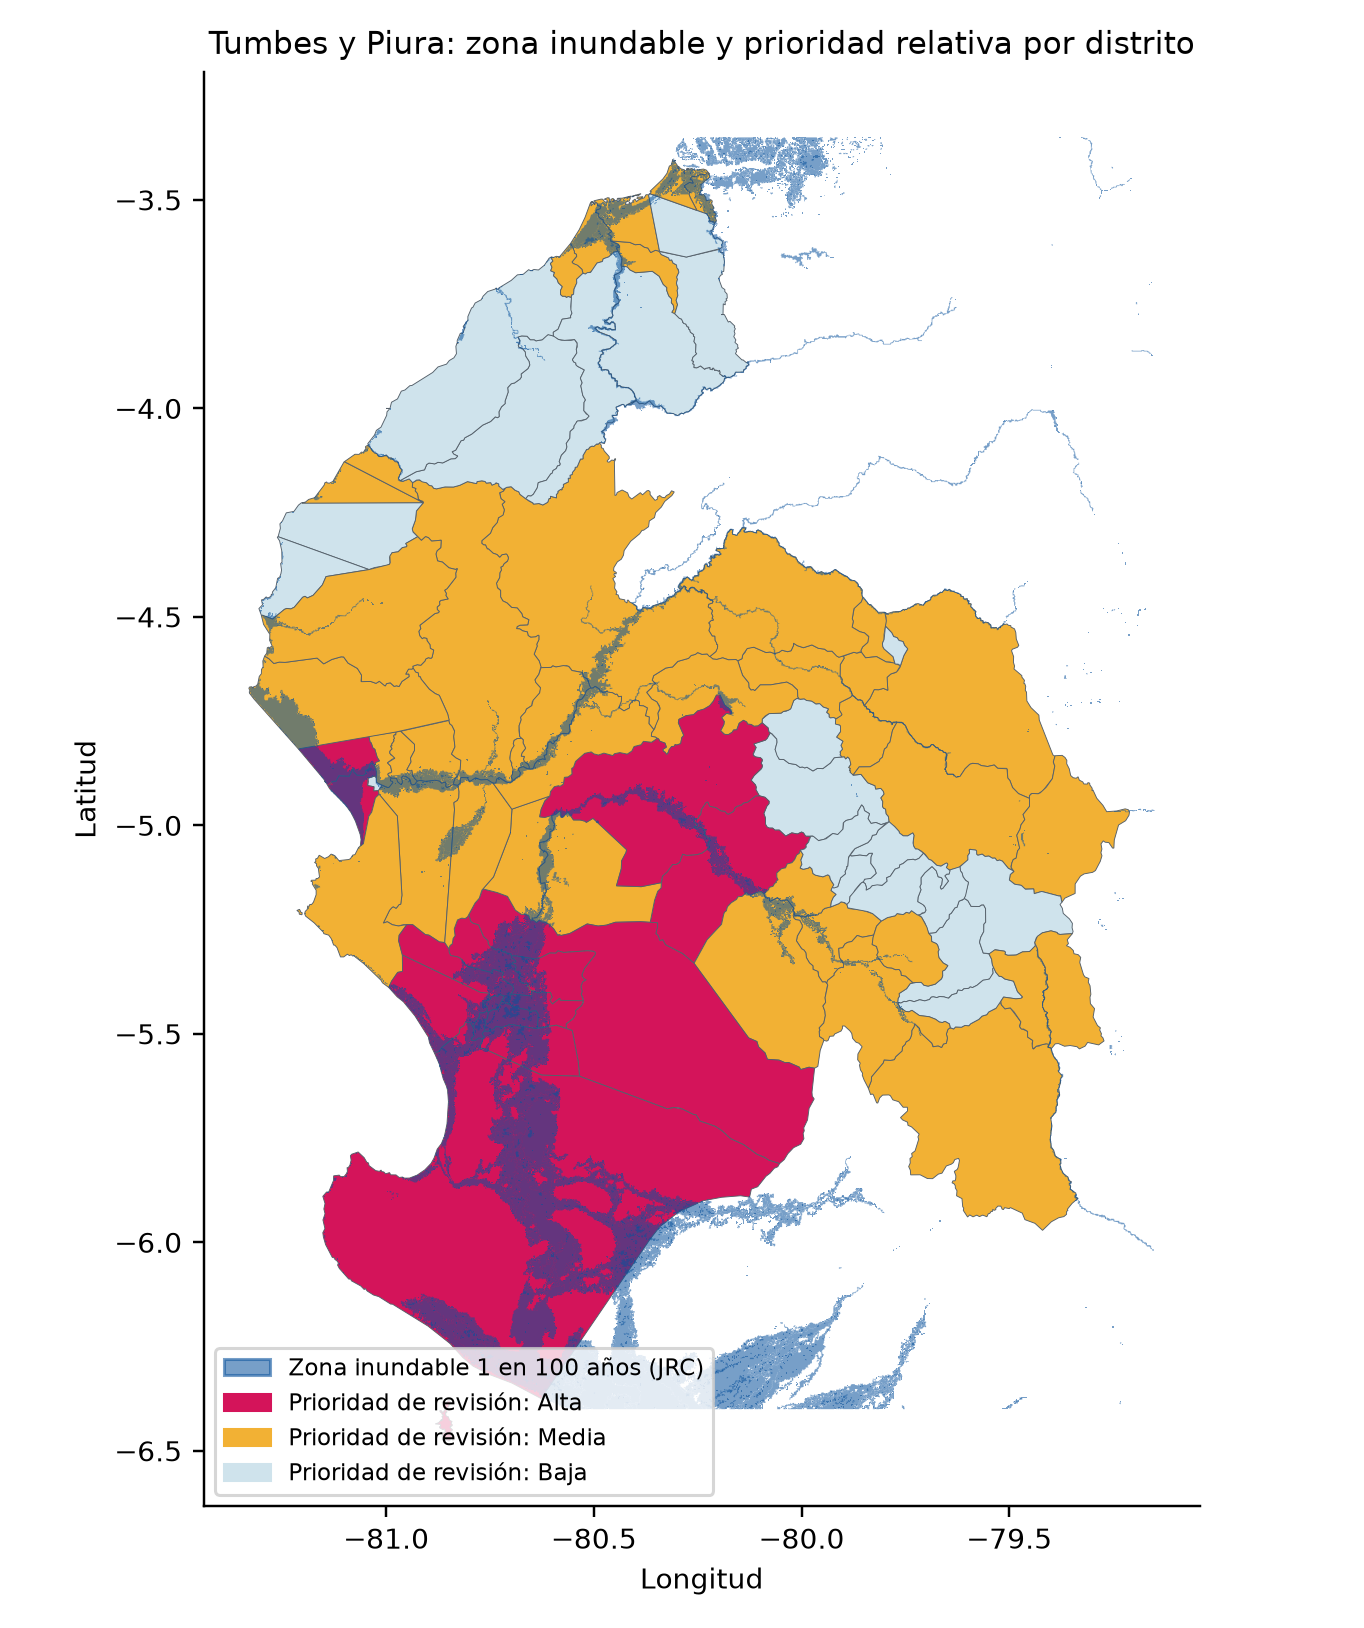
\includegraphics[width=0.66\textwidth]{figuras/mapa_prioridad.png}
\caption{Zona inundable de 1 en 100 años (JRC) y prioridad relativa de revisión por distrito. La prioridad es el promedio de los percentiles de peligro, exposición y pobreza.}\label{fig:mapa}
\end{figure}

\section{Calidad y pruebas}

Hay 38 pruebas automáticas (\cod{pytest}), todas aprobadas:
\begin{itemize}
\item \textbf{unitarias}: anillos y acumulados, umbral de Otsu, referencia del radar sin solape, reintentos, estados;
\item \textbf{de integración y consistencia geoespacial}: sumas que concilian, acumulados que crecen, UBIGEO únicos, geometrías dentro de la caja, población alineada con las edificaciones, población distrital plausible, metadatos completos;
\item \textbf{smoke test} del sitio.
\end{itemize}
En GitHub Actions, los flujos de actualización ejecutan las pruebas \emph{antes} de guardar: si las cifras salen incoherentes, se conserva el último resultado válido. También probamos el recorrido de usuario en escritorio, en celular (375 px) y sin WebGL.

\section{Machine learning}

\begin{table}[H]\centering\small
\caption{Decisión por caso de uso.}
\begin{tabularx}{\textwidth}{p{4.2cm}p{3.3cm}Y}\toprule
Caso & Decisión & Motivo \\\midrule
A. Susceptibilidad espacial & No entrenar aún & No hay etiquetas independientes; entrenar con el JRC o con el radar propio reproduciría su sesgo. \\
B. Clasificación SAR & No entrenar aún & Falta una referencia óptica o de campo. Otsu ya está implementado como diagnóstico. \\
C. Emergencia distrito-semana & Reproducido y evaluado & Hay etiquetas 2001--2015 (DesInventar/INDECI): 311 semanas positivas. \\\bottomrule
\end{tabularx}
\end{table}

\begin{figure}[H]\centering
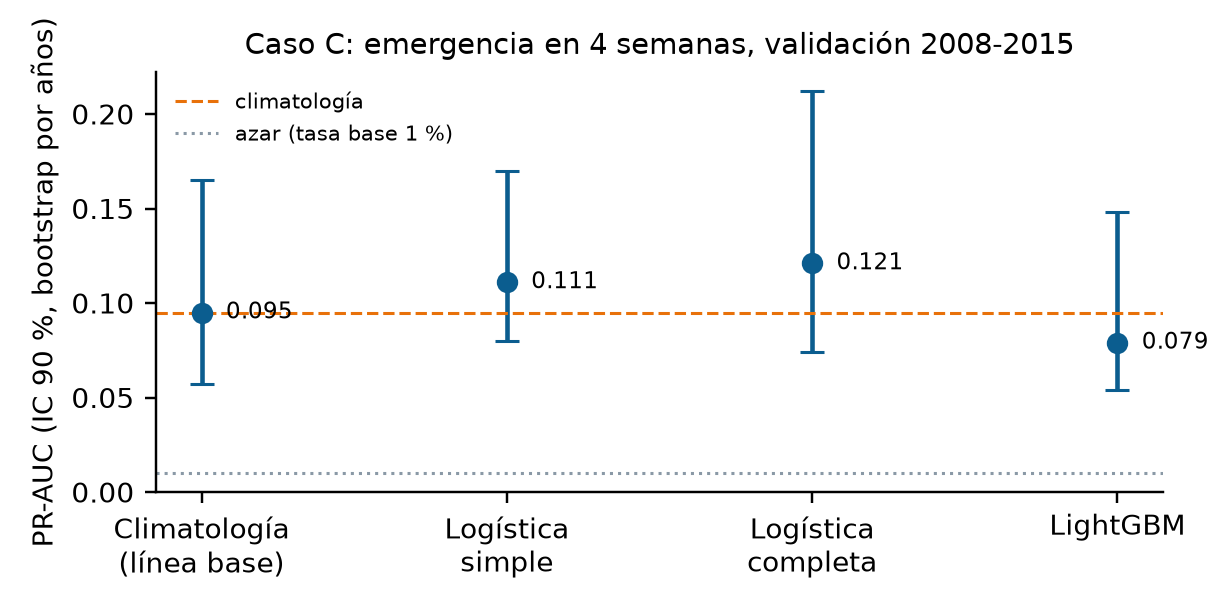
\includegraphics[width=0.78\textwidth]{figuras/ml_pr_auc.png}
\caption{PR-AUC con intervalo de confianza del 90\,\% (bootstrap de 2\,000 remuestreos por años completos). La logística simple supera a la climatología con probabilidad 0,92, pero el intervalo de la diferencia, [$-0{,}003$; $0{,}039$], incluye el cero.}
\end{figure}

\paragraph{Lectura.}
\begin{itemize}
\item La mejora sobre la climatología es posible, pero no está demostrada.
\item LightGBM no supera la línea base.
\item Las probabilidades sin calibrar no deben leerse como probabilidades: el Brier es 0,144 sin recalibrar y 0,0095 con recalibración isotónica.
\item El modelo captura el 46\,\% de las emergencias de Tumbes y solo el 5\,\% de las de Piura.
\item No se justifica usar redes profundas con esta muestra.
\end{itemize}

\section{Aporte al INEI y políticas públicas}

\paragraph{Aporte.} Proponemos una estadística territorial de población y edificaciones potencialmente expuestas por UBIGEO, con metadatos, diccionario de variables, periodicidad y gobernanza. Puede interoperar con CENEPRED, MINEDU, MINSA, ANA y SENAMHI. El INEI produce estadística; las alertas y las obras corresponden a otras entidades.

\paragraph{Políticas para evaluar.}
\begin{enumerate}
\item Continuidad educativa en los locales expuestos.
\item Continuidad de los servicios de salud.
\item Ordenamiento territorial.
\item Mantenimiento focalizado de drenes y cauces.
\item Rutas de evacuación y refugios.
\item Comunicación de riesgo.
\item Levantamiento prioritario de datos.
\end{enumerate}
Ninguna reemplaza una evaluación oficial de riesgo ni autoriza reubicaciones.

\section{Estado por componente}

\begin{longtable}{p{7.2cm}p{1.8cm}p{6.2cm}}
\toprule
Componente & Estado & Evidencia / nota \\\midrule\endhead
Auditoría técnica y de datos & \hecho & \cod{docs/01}, \cod{auditoria\_cifras.json} \\
Corrección de cifras (E1--E4, E7) & \hecho & \cod{cifras\_antes\_despues.csv}; pruebas \\
Radar reciente recalculado & \VivoEstado & \cod{data/huellas/vivo.json} \\
ETL con reintentos, registro y degradación & \hecho\ / \parcial & local probado; perfiles en línea dependen de Actions \\
Metadatos y estado por capa & \hecho & \cod{metadatos.json} \\
Mapa 2D, selectores, comparador y descargas & \hecho & recorrido en escritorio y celular \\
Panel de decisiones por UBIGEO & \hecho & \cod{panel\_distritos.csv} \\
Validación con cifras oficiales del INEI & \parcial & se usó una estimación 2020 de terceros \\
Umbral SAR adaptativo & \parcial & implementado; falta una referencia para elegirlo \\
Pruebas y CI & \hecho & 38 aprobadas \\
Machine learning (plan y experimento) & \hecho & \cod{docs/02}, \cod{ml\_evaluacion.json} \\
Aporte al INEI, bibliografía, políticas & \hecho & \cod{docs/03--05} (21 referencias verificadas) \\
Informe final en Word & \hecho & \cod{INFORME\_FINAL\_PROYECTO\_INTEGRADOR.docx} \\
Publicación en GitHub Pages & \hecho & \cod{marciashapiama.github.io/iapn-inei} \\\bottomrule
\end{longtable}

\section{Próximos pasos}

\begin{enumerate}
\item \textbf{P0}: proponer los cambios al repositorio del equipo mediante un \emph{pull request} desde el fork.
\item \textbf{P1}: obtener los límites distritales oficiales del INEI (78 distritos), el padrón ESCALE de colegios y la población oficial por distrito para validar.
\item \textbf{P2}: construir una referencia independiente de inundación para 2017 y 2023, y entrenar y validar los casos A y B por cuenca y por evento.
\item \textbf{P3}: extender el sistema a la costa norte y luego a todo el país.
\end{enumerate}

\begin{thebibliography}{99}\small
\bibitem{brena1} Breña-Aliaga, J.~C., \& Cruz-Machacuay, J. (2026). Estimación de umbrales y dinámica de inundaciones integrando Random Forest, el índice SDWI de Sentinel-1, el modelo HAND y datos SAR en la cuenca del río Tumbes. \emph{Ingeniería del Agua, 30}(3), 211--228. \url{https://doi.org/10.4995/ia.25917}
\bibitem{brena2} Breña Aliaga, J.~C., Vidal, J., Felipe, O., Bourrel, L., Rau, P., \& Lavado-Casimiro, W. (2026). Estimation of flood thresholds for hydrological warning purposes using Sentinel-1 SAR imagery-based modeling in the Tumbes River basin (Peru). \emph{Remote Sensing, 18}(10), 1493. \url{https://doi.org/10.3390/rs18101493}
\bibitem{twele} Twele, A., Cao, W., Plank, S., \& Martinis, S. (2016). Sentinel-1-based flood mapping: A fully automated processing chain. \emph{International Journal of Remote Sensing, 37}(13), 2990--3004. \url{https://doi.org/10.1080/01431161.2016.1192304}
\bibitem{tellman} Tellman, B., Sullivan, J.~A., Kuhn, C., Kettner, A.~J., Doyle, C.~S., Brakenridge, G.~R., Erickson, T.~A., \& Slayback, D.~A. (2021). Satellite imaging reveals increased proportion of population exposed to floods. \emph{Nature, 596}(7870), 80--86. \url{https://doi.org/10.1038/s41586-021-03695-w}
\bibitem{chini} Chini, M., Hostache, R., Giustarini, L., \& Matgen, P. (2017). A hierarchical split-based approach for parametric thresholding of SAR images. \emph{IEEE Transactions on Geoscience and Remote Sensing, 55}(12), 6975--6988. \url{https://doi.org/10.1109/TGRS.2017.2737664}
\bibitem{dottori} Dottori, F., Salamon, P., Bianchi, A., Alfieri, L., Hirpa, F.~A., \& Feyen, L. (2016). Development and evaluation of a framework for global flood hazard mapping. \emph{Advances in Water Resources, 94}, 87--102. \url{https://doi.org/10.1016/j.advwatres.2016.05.002}
\bibitem{tatem} Tatem, A.~J. (2017). WorldPop, open data for spatial demography. \emph{Scientific Data, 4}, 170004. \url{https://doi.org/10.1038/sdata.2017.4}
\bibitem{nearing} Nearing, G., et al. (2024). Global prediction of extreme floods in ungauged watersheds. \emph{Nature, 627}(8004), 559--563. \url{https://doi.org/10.1038/s41586-024-07145-1}
\bibitem{roberts} Roberts, D.~R., et al. (2017). Cross-validation strategies for data with temporal, spatial, hierarchical, or phylogenetic structure. \emph{Ecography, 40}(8), 913--929. \url{https://doi.org/10.1111/ecog.02881}
\bibitem{dawson} Dawson, G., Butt, J., Jones, A., \& Fraccaro, P. (2023). Flood susceptibility mapping at the country scale using machine learning approaches. \emph{Applied AI Letters, 4}(4), e88. \url{https://doi.org/10.1002/ail2.88}
\end{thebibliography}
\noindent{\small La bibliografía completa (21 referencias en APA 7, con los DOI verificados en Crossref) está en \cod{docs/04\_ESTADO\_DEL\_ARTE\_Y\_BIBLIOGRAFIA.md}.}

\end{document}
